\begin{experiment}{Ensembles dimensionality.}{\small \sffamily\textbf{Description}

We are testing dimensions on range 1---4 using 2 datasets, analyzing:

\begin{itemize}
\tightlist
	\item \texttt{MOD} --- \emph{Universal model}, an ensemble, using \textbf{random} approach, grain \emph{18}, radius \emph{0.18}, limit \emph{5}, using \textbf{lone participation}.

\end{itemize}


\textbf{Results}

\centering
	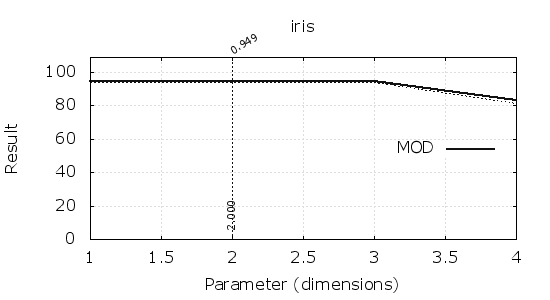
\includegraphics[width=.49\textwidth]{plots/experiment_6a_iris.png}
	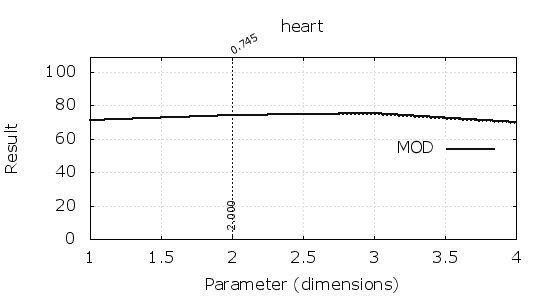
\includegraphics[width=.49\textwidth]{plots/experiment_6a_heart.png}
	\captionof{figure}{Ensembles dimensionality.}
	\label{fig:experiment_6a}
}\end{experiment}